\documentclass[a4paper,10pt]{article}
%\VignetteIndexEntry{useR 2008 abstract}

\usepackage{url}
\usepackage{Sweave}


\title{R4X: Convenient XML Manipulation for R}
\author{Romain Francois - Mango Solutions \\
\url{rfrancois@mango-solutions.com}}

\begin{document}

\maketitle

\begin{abstract}
The R4X package enhances the \texttt{XML} package by 
providing a simple mechanism to create, read and manipulate XML structures 
from within R. The functionality of the package is based on the E4X (EcmaScript for XML)
add-on to the javascript specifications. 

R4X implements templating of XML structures based on the \texttt{brew} package
and convenient extraction of XML content using an XPath-like syntax. 

The XML format is used to transfer data accross many applications, specially web applications. The R4X 
package came from the need of a convenient tool to manipulate XML data when R is part of a bigger application. 
The presentation will describe key features of the R4X package, including examples of using
the functionality to build a simple RSS reader and a tag cloud generated by using description 
of all current CRAN packages.

\end{abstract}

\textbf{Keywords}: XML, templates, data manipulation

\subsection*{Creation of XML}

The generic \texttt{xml} function allows creation of XML structures as defined by the \texttt{XML} package
from character vectors, connections. Users can write other \texttt{xml} methods to convert 
different formats to XML structures

\begin{Schunk}
\begin{Sinput}
R> x <- xml( '
     <test>
        <foo blah="1"/>
        <bar/>
     </test>' ) 
R> x
\end{Sinput}
\begin{Soutput}
<test>
 <foo blah="1"/>
 <bar/>
</test>
\end{Soutput}
\begin{Sinput}
R> class( x) 
\end{Sinput}
\begin{Soutput}
[1] "XMLNode"
\end{Soutput}
\end{Schunk}

The character string used by the \texttt{xml} function may contain R code embedded in curly brackets.

\begin{Schunk}
\begin{Sinput}
R> y <- "something"
R> x <- xml( '
     <test>
        <foo blah="{y}"/>
        <bar/>
     </test>' ) 
R> x
\end{Sinput}
\begin{Soutput}
<test>
 <foo blah="something"/>
 <bar/>
</test>
\end{Soutput}
\end{Schunk}

\subsection*{Extracting XML content}

The \texttt{[} and \texttt{[[} methods from the \texttt{XML} package are masked by R4X to 
provide an XPath-like mechanism for extracting and modifying content of an XML structure.

\begin{Schunk}
\begin{Sinput}
R> x <- xml( '
   <root>
     <child id="1">
       <subchild id = "sub1" >foo</subchild>
       <subchild id = "sub2" >bar</subchild>
     </child>
     <child id="2">
       <subchild id="a">blah</subchild>
       <subchild id="b">bob</subchild>
       <something id="c" />
     </child>
     <fruits>
        <fruit>banana</fruit>
        <fruit>mango</fruit>
     </fruits>
   </root>  
   ' )
R> # extracting a single XMLNode
R> x[ "fruits" ]   
\end{Sinput}
\begin{Soutput}
<fruits>
 <fruit>banana</fruit>
 <fruit>mango</fruit>
</fruits>
\end{Soutput}
\begin{Sinput}
R> # extracting the text content of each <subchild>
R> x[ "child/subchild/#" ]  
\end{Sinput}
\begin{Soutput}
child.subchild child.subchild child.subchild child.subchild 
         "foo"          "bar"         "blah"          "bob" 
\end{Soutput}
\begin{Sinput}
R> # extracting the id attribute of each <child>
R> x[ "child/@id" ]   
\end{Sinput}
\begin{Soutput}
child child 
  "1"   "2" 
\end{Soutput}
\begin{Sinput}
R> # extracting the <subchild> of the second <child>
R> x[ "child[2]/subchild" ]      
\end{Sinput}
\begin{Soutput}
$subchild
<subchild id="a">blah</subchild>

$subchild
<subchild id="b">bob</subchild>
\end{Soutput}
\end{Schunk}

\subsection*{Example - Tag Cloud Generator}

\begin{figure}[h]
 \centering
 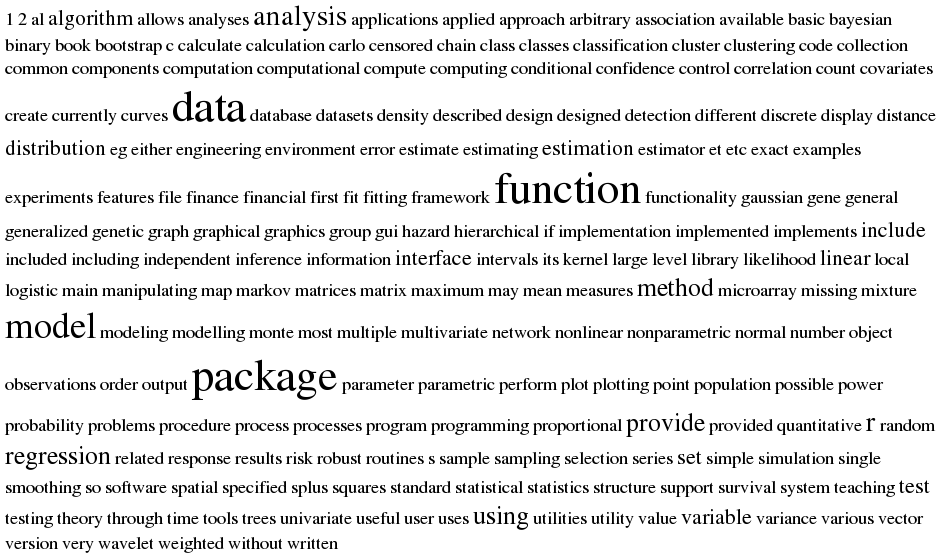
\includegraphics[width=.9\textwidth]{pictures/tags.png}
 \caption{Tag cloud generated from words used in descriptions of CRAN packages using the R4X package. }
\end{figure}


\end{document}
